\documentclass[a4paper, 12pt]{article}%тип документа

%отступы
\usepackage[left=2cm,right=2cm,top=2cm,bottom=3cm,bindingoffset=0cm]{geometry}
\setlength{\parindent}{5ex}

%Русский язык
\usepackage[T2A]{fontenc} %кодировка
\usepackage[utf8]{inputenc} %кодировка исходного кода
\usepackage[english,russian]{babel} %локализация и переносы

%Вставка картинок
\usepackage{graphicx}
\graphicspath{{pictures/}}
\DeclareGraphicsExtensions{.pdf,.png,.jpg}

%Графики
\usepackage{pgfplots}
\pgfplotsset{compat=1.9}

%Математика
\usepackage{amsmath, amsfonts, amssymb, amsthm, mathtools}

%Таблицы
\usepackage{longtable} 
\usepackage{float}

%Римские цифры
\newcommand{\RomanNumeralCaps}[1]{\uppercase\expandafter{\romannumeral#1}}

\usepackage{multirow}


\begin{document}
	\begin{titlepage}
		\begin{center}
			\textsc{Федеральное государственное автономное образовательное учреждение высшего образования«Московский физико-технический институт (национальный исследовательский университет)»\\[5mm]
			}
			
			\vfill
			
			\textbf{Отчёт по лабораторной работы 2.1.6\\[3mm]
				Эффект Джоуля - Томсона.
				\\[50mm]
			}
			
		\end{center}
		
		\hfill
		\begin{minipage}{.5\textwidth}
			Выполнил студент:\\[2mm]
			Сериков Василий Романович\\[2mm]
			группа: Б03-102\\[5mm]
			
		\end{minipage}
		\vfill
		\begin{center}
			Москва, 2022 г.
		\end{center}
		
	\end{titlepage}
	
	\newpage
	\textbf{Аннотация}\\
	
	
	\textbf{Цель работы: }\\
	
	Определение изменения температуры углекислого газа при протекании через малопроницаемую перегородку при разных начальных значениях давления и температуры; 2) вычисление по результатам опытов коэффициентов Ван-дер-Ваальса «a» и «b».\\
	
	
	\textbf{Теоретические сведения: } \\
	
	Эффектом Джоуля–Томсона называется изменение температуры газа, медленно протекающего из области высокого в область низкого давления в условиях хорошей тепловой изоляции. В разреженных газах, которые приближаются по своим свойствам к идеальному газу, при таком течении температура газа не меняется. Эффект Джоуля–Томсона демонстрирует отличие исследуемого газа от идеального.\\
	
	\begin{figure}[h!]
		\centering{
			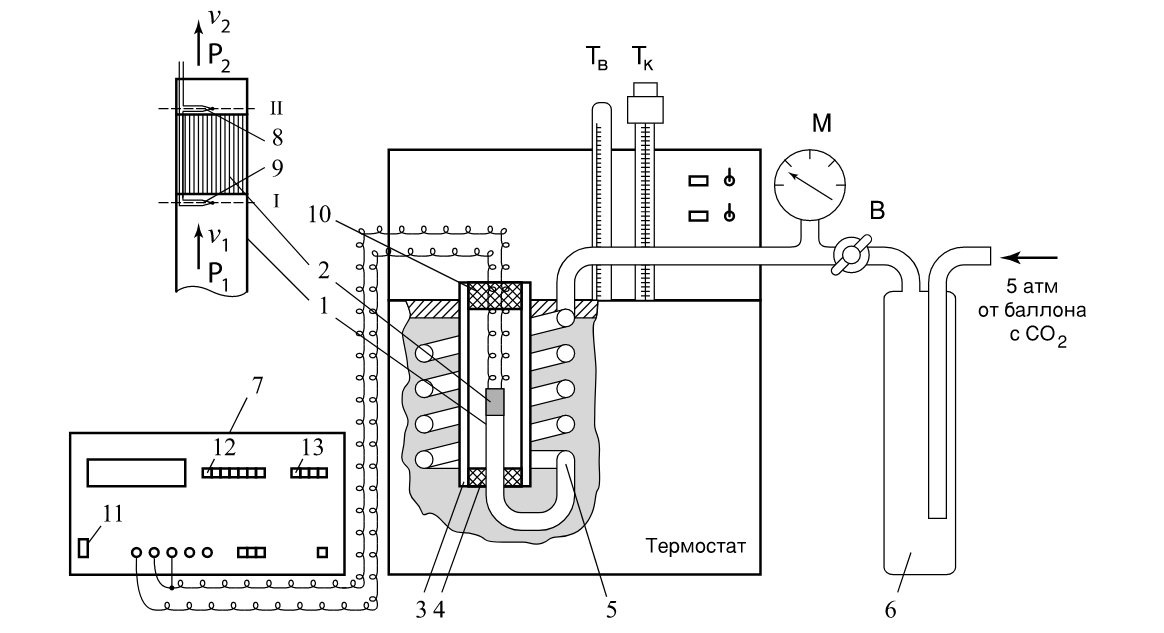
\includegraphics[width=15cm]{scheme.png}
		}
		\caption{Схема установки для изучения эффекта Джоуля–Томсона.}
	\end{figure}
	
	В работе исследуется изменение температуры углекислого газа при медленном его течении по трубке с пористой перегородкой (рис. 1). Трубка 1 хорошо теплоизолирована. Газ из области повышенного давления $P_1$ проходит через множество узких и длинных каналов пористой перегородки 2 в область с атмосферным давлением $P_2$. Перепад давления $\Delta P = P_1 - P_2$ из-за большого сопротивления каналов может быть заметным даже при малой скорости течения газа в трубке. Величина эффекта Джоуля–Томсона определяется по разности температуры газа до и после перегородки.\\
	
	Рассмотрим стационарный поток газа между произвольными сечениями I и II трубки (до перегородки и после нее). Пусть, для определенности, через трубку прошел 1 моль углекислого газа; $\mu$ --- его молярная масса. Молярные объемы газа, его давления и отнесенные к молю внутренние энергии газа в сечениях I и II обозначим соответственно $V_1, P_1, U_1$ и $V_2, P_2, U_2$. Для того чтобы ввести в трубку объем $V_1$, над газом нужно совершить работу $A_1 = P_1V_1$. Проходя через сечение II, газ сам совершает работу $A_2 = P_2V_2$. Так как через боковые стенки не происходит ни обмена теплом, ни передачи механической энергии, то:
	
	\begin{equation}
		A_1 - A_2 = \left(U_2 + \dfrac{\mu v_2^2}{2}\right) - \left(U_1 + \dfrac{\mu v_1^2}{2}\right).
	\end{equation}
	
	В уравнении (1) учтено изменение как внутренней (первые члены в скобках), так и кинетической (вторые члены в скобках) энергии газа. Подставляя в (1) написанные выражения для $A_1$ и $A_2$ и перегруппировывая члены, найдем:
	
	\begin{equation}
		H_1 - H_2 = (U_1 + P_1V_1) - (U_2 + P_2V_2) = \dfrac{1}{2} \mu (v_2^2 - v_1^2).
	\end{equation}
	
	Сделаем несколько замечаний. Прежде всего отметим, что в процессе Джоуля–Томсона газ испытывает в пористой перегородке существенное трение, приводящее к ее нагреву. Потери энергии на нагрев трубки в начале процесса могут быть очень существенными и сильно искажают ход явления. После того как температура трубки установится и газ станет уносить с собой все выделенное им в пробке тепло, формула (1) становится точной, если, конечно, теплоизоляция трубки достаточно хороша и не происходит утечек тепла наружу через ее стенки.\\
	
	Второе замечание связано с правой частью (2). Процесс Джоуля–Томсона в чистом виде осуществляется лишь в том случае, если правой частью можно пренебречь, т. е. если макроскопическая скорость газа с обеих сторон трубки достаточно мала. У нас сейчас нет критерия, который позволил бы установить, когда это можно сделать. Поэтому мы отложим на некоторое время обсуждение вопроса о правой части (2), а пока будем считать, что энтальпия газа не меняется.
	
	\begin{equation}
		\mu_{\text{Д-Т}} = \dfrac{\Delta T}{\Delta P} \approx \dfrac{\frac{2a}{RT}-b}{C_p}.
	\end{equation}
	
	Отсюда видно, что эффект Джоуля–Томсона для не очень плотного газа зависит от соотношения величин $a$ и $b$, которые оказывают противоположное влияние на знак эффекта. Если силы взаимодействия между молекулами велики, так что превалирует <<поправка на давление>>, то основную роль играет член, содержащий $a$, и
	
	\begin{equation}
		\dfrac{\Delta T}{\Delta P} > 0,
	\end{equation}
	
	то есть газ при расширении охлаждается ($\Delta T < 0$, так как всегда $\Delta P < 0$). В обратном случае (малые $a$)
	
	\begin{equation}
		\dfrac{\Delta T}{\Delta P} < 0,
	\end{equation}
	то есть газ нагревается ($\Delta T > 0$, так как по-прежнему $\Delta P < 0$).\\
	Этот результат нетрудно понять из энергетических соображений. Как мы уже знаем, у идеального газа эффект Джоуля–Томсона отсутствует. Идеальный газ отличается от реального тем, что в нем можно пренебречь потенциальной энергией взаимодействия молекул. Наличие этой энергии приводит к охлаждению или нагреванию реальных газов при расширении. При больших $a$ велика энергия притяжения молекул. Это означает, что потенциальная энергия молекул при их сближении уменьшается, а при удалении --- при расширении газа --- возрастает. Возрастание потенциальной энергии молекул происходит за счет их кинетической энергии --- температура газа при расширении падает. Аналогичные рассуждения позволяют понять, почему расширяющийся газ нагревается при больших значениях $b$.\\
 $$ T_i = 2a/Rb$$	Как следует из формулы выше при температуре $T_i$ коэффициент $\mu_{\text{Д-Т}} $ обращается в нуль. Используя связь между коэффициентами $a$ и $b$ и критической температурой, найдем
	\begin{equation}
		T_{\text{инв}} = \dfrac{27}{4}T_{\text{кр}}.
	\end{equation}
	
	
	При температуре $T_{\text{инв}}$ эффект Джоуля–Томсона меняет знак: ниже температуры инверсии эффект положителен ($\mu_{Д-Т} > 0$, газ охлаждается), выше $T_{\text{инв}}$ эффект отрицателен ($\mu_{\text{Д-Т}} < 0$, газ нагревается).\\
	
%	Температура инверсии у всех газов лежит значительно выше критической. Для большинства газов $T_{\text{инв}}/T_{\text{кр}} = 5-8$. Например, для гелия $T_{инв} = 46$К, $T_{кр} = 5,2$К; для водорода $T_{инв} = 205$К,$ T_{кр }= 33$К; для азота $T_{инв} = 604$ К, $T_{кр} = 126$ К; для воздуха $T_{инв} = 650$ К, $T_{кр} = 132,6 $К; для углекислого газа $T_{инв} = 2050$ К, $T_{кр} = 304$ К. Температура инверсии у гелия и водорода значительно ниже комнатной, поэтому при обычных температурах эти газы при расширении нагреваются. Температура инверсии остальных газов выше комнатной, и при нормальных условиях температура при расширении газа падает.\\
	
%	Сравнивая приведенные значения $T_{\text{инв}}$ и $T_{\text{кр}}$, можно убедиться в том, что предсказания, следующие из формулы Ван-дер-Ваальса, у реальных газов выполняются не очень хорошо. Правильно передавая качественную картину поведения реальных газов, формула Ван-дер-Ваальса не претендует на хорошее количественное описание этой картины.\\
	
	При больших изменениях давления, например, при дросселировании от 200 до 1 атм (интегральный эффект Джоуля–Томсона), как это нередко бывает в промышленных установках, разложением  пользоваться нельзя и приходится прибегать к общему соотношению . При этом связь между температурой и давлением находится с помощью специальных диаграмм, например, кривых $H = const$, проведенных в координатах температура-давление или температура-энтропия. Такие диаграммы строятся по экспериментальным данным и широко используются в технике.\\
	
	Вернемся к влиянию правой части уравнения (2) на изменение температуры расширяющегося газа. Для этого сравним изменение температуры, происходящее вследствие эффекта Джоуля–Томсона, с
	изменением температуры, возникающим из-за изменения кинетической энергии газа . Увеличение кинетической энергии газа вызывает заметное и приблизительно одинаковое понижение его температуры как у реальных, так и у идеальных газов. Поэтому при оценках нет смысла пользоваться сложными формулами для газа Ван-дер-Ваальса.\\
	
	Заменяя в формуле (2) $U$ через $C_V T$ и $P V$ через $RT$, найдем
	
	\begin{equation}
		(R+C_V)(T_1 - T_2) = \mu(v_2^2 - v_1^2)/2,
	\end{equation}
	или
	\begin{equation}
		\Delta T = \dfrac{\mu}{2C_p} (v_2^2 - v_1^2).
	\end{equation}
	
	В условиях нашего опыта расход газа $Q$ на выходе из пористой перегородки не превышает 10 $см^3/с$, а диаметр трубки равен 3 мм. Поэтому
	
	\begin{equation}
		v_2 \leqslant \dfrac{4Q}{\pi d^2} \approx 140 \text{см/с}.
	\end{equation}
	Скорость $v_1$ газа у входа в пробку относится к скорости $v_2$ у выхода из нее как давление $P_2$ относится к $P_1$. В нашей установке $P_1$ = 4 атм, a $P_2$ = 1 атм, поэтому
	\begin{equation}
		v_1 = \dfrac{P_2}{P_1} v_2 = 35 \text{см/с}.
	\end{equation}
	Для углекислого газа $\mu$ = 44 г/моль, $C_p$ = 40 Дж/($моль \cdot К$); имеем
	\begin{equation}
		\Delta T = \dfrac{\mu}{2C_p} (v_2^2 - v_1^2) = 7 \cdot 10^{-4}\text{ К}.
	\end{equation}
	Это изменение температуры ничтожно мало по сравнению с измеряемым эффектом (несколько градусов).\\
	В данной лабораторной работе исследуется коэффициент дифференциального эффекта Джоуля–Томсона для углекислого газа. По экспериментальным результатам оценивается коэффициент теплового расширения, постоянные в уравнении Ван-дер-Ваальса и температура инверсии углекислого газа. Начальная температура газа $T_1$ задается термостатом. Измерения проводятся при трех температурах: комнатной, $50 С$ и $80 С$.\\
	
	
	
	\textbf{Экспериментальная установка.}\\
	
	
	Схема установки для исследования эффекта Джоуля–Томсона в углекислом газе см. рис. 1. Основным элементом установки является трубка 1 с пористой перегородкой 2, через которую пропускается исследуемый газ. Трубка имеет длину 80 мм и сделана из нержавеющей стали, обладающей, как известно, малой теплопроводностью. Диаметр трубки $d = 3$ мм, толщина стенок $0,2$ мм. Пористая перегородка расположена в конце трубки и представляет собой стеклянную пористую пробку со множеством узких и длинных каналов. Пористость и толщина пробки ($l = 5$ мм) подобраны так, чтобы обеспечить оптимальный поток газа при перепаде давлений $\Delta P  $ 4 атм (расход газа составляет около 10 $см^3/с$); при этом в результате эффекта Джоуля–Томсона создается достаточная разность температур.\\
	
	Углекислый газ под повышенным давлением поступает в трубку через змеевик 5 из балластного баллона 6. Медный змеевик омывается водой и нагревает медленно протекающий через него газ до температуры воды в термостате. Температура воды измеряется термометром $T$в, помещенным в термостате. Требуемая температура воды устанавливается и поддерживается во время эксперимента при помощи контактного термометра $T$к.
	Давление газа в трубке измеряется манометром М и регулируется вентилем В (при открывании вентиля В, то есть  при повороте ручки против часовой стрелки, давление $P_1$ повышается). Манометр М измеряет разность между давлением внутри трубки и наружным (атмосферным) давлением. Так как углекислый газ после пористой перегородки выходит в область с атмосферным давлением $P_2$, то этот манометр непосредственно измеряет перепад давления на входе и на выходе трубки $\Delta P = P1 - P2.$\\
	Разность температур газа до перегородки и после нее измеряется дифференциальной термопарой медь-константан. Константановая проволока диаметром 0,1 мм соединяет спаи 8 и 9, а медные проволоки (того же диаметра) подсоединены к цифровому вольтметру 7. Отвод тепла через проволоку столь малого сечения пренебрежимо мал. Для уменьшения теплоотвода трубка с пористой перегородкой помещена в трубу Дьюара 3, стенки которой посеребрены, для уменьшения теплоотдачи, связанной с излучением. Для уменьшения теплоотдачи за счет конвекции один конец трубы Дьюара уплотнен кольцом 4, а другой закрыт пробкой 10 из пенопласта. Такая пробка практически не создает перепада давлений между внутренней полостью трубы и атмосферой.\\
	
	
	\textbf{Используемое оборудование: }\\
	
	Трубка с пористой перегородкой; труба Дьюара; термостат; термометры; дифференциальная термопара; микровольтметр; балластный баллон; манометр.\\
	
	
	
	\textbf{Результаты измерений и обработка данных: }\\
	
	\begin{enumerate}
		
		\item Начальные данные и погрешности: $\sigma_P = 0.1$ атм., $\sigma_U = 1$ мкВ 
	
	\item Проведем измерение показаний вольтметра в зависимости от давления для различных температур. Полученные данные занесем в таблицу ($\sigma_{\Delta T} =\Delta T \sigma_P/\Delta P \approx 0,03 ^\circ C$)
	
	\begin{longtable}{|c|c|c|c|c|c|c|}
		\hline
	$\Delta P$, атм & $U$, мкВ  & $\Delta T, ^\circ C$  &   &$\Delta P$, атм  &  $U$, мкВ   & $\Delta T, ^\circ C$  \\ \hline
		4 &  126  & 3,09 &    &  4  &  123  & 3,02  \\ \hline
		3,5 &  108  & 2,65 &    & 3,5   &  105  &  2,58 \\ \hline
		3  &  89  &  2,18 &    &  3  &  83  &  2,04 \\ \hline
		2,5 &  61  & 1,50  &    &  2,5  &  70  & 1,72 \\ \hline
		\caption{Данные для Т = 296 К, Т = 301 К}
	\end{longtable}
	
	
		\begin{longtable}{|c|c|c|c|c|c|c|}
		\hline
		$\Delta P$, атм & $U$, мкВ  & $\Delta T, ^\circ C$  &   &$\Delta P$, атм  &  $U$, мкВ   & $\Delta T, ^\circ C$  \\ \hline
		4 &  124  &  2,98 &    &  4  &  113  &  2,66 \\ \hline
		3,5 &  98  &  2,36 &    & 3,5   &  95  & 2,24  \\ \hline
		3  &  86  & 2,07 &    &  3  &  73  & 1,72 \\ \hline
		2,5 &  57  & 1,37  &    &  2,5  & 52 & 1,22 \\ \hline
		\caption{Данные для Т = 306 К, Т = 316 К}
	\end{longtable}

\newpage

	\item Построим график зависимости $\Delta T (\Delta P)$ По наклону графика определим коэффициент Джоуля-Томсона для каждой температуры. По МНК определим погрешности полученных коэффициентов.($\sigma_{\mu} = 0,3$ К/МПа)
	
		\begin{figure}[h!]
		\centering{
			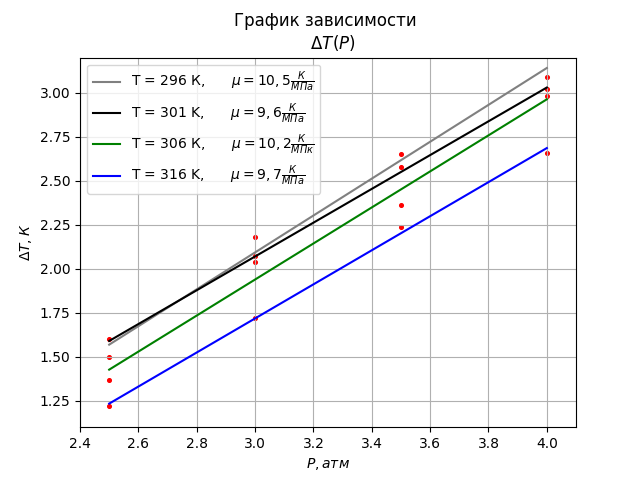
\includegraphics[width=15cm]{lab 2_1_6.png}
		}
	\end{figure}
	
	
	\item Определим постоянные $a$, $b$ и $T_{\text{инв}}$ для углекислого газа для наших температур по формулам: 
	
	$$\mu_{\text{Д-Т}} =  \dfrac{\frac{2a}{RT}-b}{C_p}$$ 
	
	$$a = \dfrac{2R^2(\mu_2 - \mu_1)}{ \left( \dfrac{1}{T_1} - \dfrac{1}{T_2} \right)}  $$
	
	$$ b = \dfrac{2a}{RT_1} - 4R \mu_1  $$
	
	$$ T_{\text{инв}} = 2a/Rb $$
	\begin{longtable}{|c|c|c|}
		\hline
		T, K & 306 - 296 & 316 - 306\\
		\hline
		a, Н м$^4$/моль$^2$ & 0.38 $\pm 0.04$& 0,668 $\pm 0.04$\\
		\hline
		b, см$^3$/моль & 44 $\pm 5$& $ 44\pm 5$\\
		\hline
		$T_{\text{инв}}$, К& 2046 $\pm 232$& 3645 $\pm 414$\\
		\hline
	\end{longtable}

\newpage

	\end{enumerate}

	\textbf{Обсуждение результатов: }\\
	В ходе данной работы мы определили коэффициенты уравнения газа  Ван-дер-Ваальса, одна пара из которых совпадает с теоретическими результатами(a = 0,3652Н м$^4$/моль$^2$, b = 42,79 см$^3$/моль, $T_{\text{инв}}$ = 2052 К) в пределах погрешности, а вторая нет. Аналогично с температурой инверсии в первом и втором случае.  


\textbf{Выводы: }\\
По полученным результатам нельзя однозначно установить применимость уравнения газа  Ван-дер-Ваальса. Необходимо более точно проводить эксперимент, используя более точные методы и приборы. Основная проблема проведения эксперимента - определение момента, когда можно считать, что система пришла в равновесие, отсюда и следует большой разброс полученных значений.


	\end{document}
	